\documentclass[12pt,twocolumn]{article}

\usepackage{usenix}
\usepackage[utf8]{inputenc}
\usepackage{setspace}
\usepackage{hyperref}
\usepackage{graphicx}

\hypersetup{
    bookmarks=true,         % show bookmarks bar?
    unicode=false,          % non-Latin characters in Acrobat’s bookmarks
    pdftoolbar=true,        % show Acrobat’s toolbar?
    pdfmenubar=true,        % show Acrobat’s menu?
    pdffitwindow=false,     % window fit to page when opened
    pdfstartview={FitH},    % fits the width of the page to the window
    pdftitle={My title},    % title
    pdfauthor={Author},     % author
    pdfsubject={Subject},   % subject of the document
    pdfcreator={Creator},   % creator of the document
    pdfproducer={Producer}, % producer of the document
    pdfkeywords={keyword1} {key2} {key3}, % list of keywords
    pdfnewwindow=true,      % links in new window
    colorlinks=false,       % false: boxed links; true: colored links
    linkcolor=red,          % color of internal links (change box color with linkbordercolor)
    citecolor=green,        % color of links to bibliography
    filecolor=magenta,      % color of file links
    urlcolor=cyan           % color of external links
}

%\title{CSCI 339 OpenBazaar}
\title{\bf \sc OpenBazaar: \\ an online peer-to-peer market}

\author{
    {\rm Kevin Chen '15} \\
    {\tt kmc3}
    \and 
    {\rm Aaron Taylor '16} \\
    {\tt amt4}
}

\date{May 2014}




\begin{document}

\maketitle

\doublespacing



% % % % % % % % % % % % % % % % % % % % % % % %
% % % % % % % % % % % % % % % % % % % % % % % %
% % % % % % % % % % % % % % % % % % % % % % % %
% % % % % % % % % % % % % % % % % % % % % % % %
% % % % % % % % % % % % % % % % % % % % % % % %
% % % % % % % % % % % % % % % % % % % % % % % %
\section{Introduction}
In October 2013, the FBI was able to shut down the Silk Road, an online black market, with the seizure of a single server. They were able to 
To circumvent the problem of a single point of failure, the winners of a hackathon recently unveiled a proof-of-concept for a peer-to-peer version of the Silk Road.

Known as OpenBazaar (formerly the DarkMarket), this service incorporates many of the same user experience paradigms as its predecessor: private communication between buyers and sellers, HTML pages to view sellers' wares, a reputation system for ratings and reviews, and an arbiter-escrow feature that ensures a ``fair'' outcome when deals go sour. Each piece of the system is covered with layers of encryption, based on the bitcoin protocols and elliptic curve cryptography, to ensure that all communications are secure, all transactions are properly mediated, and all identities are correctly verified.
Still nascent, OpenBazaar has yet to implement several features that would enable the service to enter production mode and be delivered to users.

As the current system currently stands, in order for a seller to maintain a page, they basically need to maintain an active server with a fixed IP address that other users of the network can connect to in order to view their product offerings and initiate transactions. This is less than ideal for a number of reasons. What has lead to the sucess of other online marketplace systems such as eBay, Craigslist, and even the silk road, was or is the ease with which users can post post items for sale and oder items from other sellers. The current system has a large amount of setup due to the direct peer-to-peer nature of the system. We wanted to emulate the convenience and simplicity of an environment hosted on a central server within the peer to peer network. We worked on scheiving this by replicating user sites across the network using a distributed hash table with data replication to consistently determine their location.

In order for this system to work, the data for a seller's marketplace and ratings should be replicated across several nodes, the data must maintain its integrity and be mutable only by the person who published it, and it must be able to be accessed quickly by the users of the system.

We intend to implement a system of replication that brings two main advantages.
First, it would allow users the convenience of not having to keep their server up constantly if they want buyers to see their wares.
Second, it increases availability: in the event that a seller's machine or otherwise needs to go offline, his or her marketplace is being hosted by other nodes in the P2P network.

Replication also has two downsides.
First, we must ensure that when Bob requests data for Alice's market, he receives the most up-to-date version of her market. We address the challenge of synchronization later.
Second, replication disincentivizes users from maintaining their servers. That is, what is to stop Bob from powering down or disconnecting his machine with great frequency if Alice is hosting his marketplace for him? We address this problem by giving users with greater hosting uptime in the network certain perks and community incentives, such as paying smaller commissions to the third party arbiter during transactions, and positive or negative indicators in the reviews section attached to each user.

\section{How it works}
A user downloads the market software, which runs a daemon in the background and allows a user to become a node in a distributed network with a P2P library known as ZeroMQ. 

For Alice to become a seller, she can edit an HTML file designated as her seller page.
Then a buyer like Bob can browse the market, which he runs via web browser.
Bob can search for a user's nickname or click on another user's node.\footnote{At the moment, there is no functionality for searching for user nicknames, and there is a lack of anonymity since Bob must click on Alice's bare IP address if he wishes to view her wares.}

If Bob sees something he wants to buy, he sends a message to Alice.
If Alice wishes to engage in trade, an arbiter must be selected to settle disputes in the event that the deal falls through.
An arbiter may be selected from overlap between Alice's and Bob's list of approved arbiters, or randomly if their lists don't intersect.

Having selected an arbiter, the system creates a new ``multisignature'' Bitcoin address from the three users' public encryption keys.
During the duration of the transaction, this Bitcoin address holds the buyer's money in escrow.
The transaction is complete when two out of the three parties agree on where the money should go.
If everything goes smoothly and the product is shipped to the buyer, both buyer and seller sign a transaction to move the bitcoins out of escrow and into the seller's account.
If the product is defective or never ships, the arbiter must step in.

Finally, each participant rates all other participants.
Ratings are cryptographically signed with the rater's private key, which prevents users from forging reviews.
Sellers with better ratings will naturally attract more buyers. 

\section{Architectural Overview}
The \href{https://github.com/OpenBazaar/OpenBazaar}{{\tt OpenBazaar} repository} is incipient but constantly being updated.
Currently, the only supported features are the ability to connect to the distributed marketplace and the ability to view your market in the browser; transactions, ratings, and arbitrations are not possible.
Furthermore, the data for the marketplace is stored persistently with a user-created MongoDB database.
However, we would like to ensure the availability of every user's marketplace by spreading out data.
This is done with a distributed hash table (DHT), which provides fault tolerance, scalability, and decentralized autonomy.

\subsection{What is a DHT?}
\newcommand{\kv}{}
\def\kv/{$\langle$key,value$\rangle$}
A DHT is just a distributed dictionary; that is, hash table buckets are nodes across a network.
Just like any other lookup service, it maps keys to values.
In this case, the keys are hashed files or hashed file locations, and the values are the files themselves.
That is, given some key $k = hash(filename)$, the DHT should be able to figure out which node hosts \emph{filename}, thereby allowing other nodes to request that specific file.
This is shown in Figure~\ref{DHT}.

\begin{figure}[h!]
  \centering
  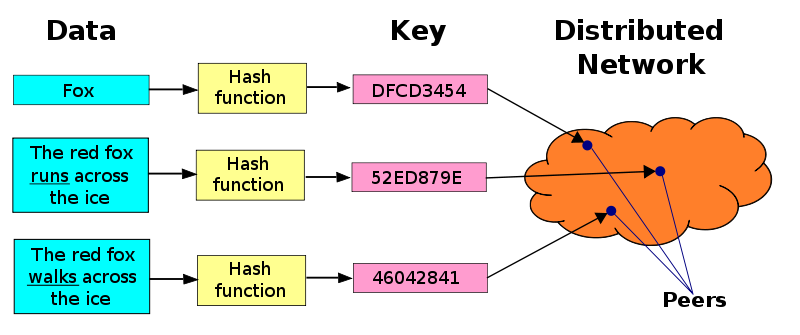
\includegraphics[width=0.5\textwidth]{images/DHT.png}
  \caption{\label{DHT}}
\end{figure}

So how do we map $hash(filename)$ to an actual node? 
In most DHTs, each node has a 160-bit identifier that determines which potential keys each node owns.\footnote{Keys and node IDs are 160 bits for consistency with the SHA-1 hash function. Nothing stops us from using a different hash function.}
Specifically, a node $n$ owns a key $k$ if $n$ is the closest node to $k$.
``Nearness'' is computed by a distance function $\delta(k, n)$, which varies depending on the DHT.

When deploying a distance function, one of the main considerations is load balancing.
Ideally, the keyspace is partitioned evenly between all the nodes in the network, so one node doesn't store more keys than another. If this is not the case, then that node can get bogged down, and the entire system will suffer in performance.

This form of consistent hashing ensures that when a node is added or removed from a system, only the keys owned by adjacent nodes are changed. 
When a node joins the system, it takes responsibility for some of its neighbor's keys.
When a node crashes or leaves the system, the keys mapping to the data it held must be allocated to new nodes.
Moreover, the more nodes are in a system, the fewer keys have to be remapped on every node entry or exit.
This is yet another advantage a DHT holds over a traditional hash table, which remaps its entire keyspace when a bucket is added or removed.



\subsection{Why Kademlia?}

\subsubsection{Unique Features}
There are many different kinds of DHTs out there. They differ in the size of their address space (128- or 160-bit keys?), in the type of hash function is used (SHA-1, SHA-2, etc.), in what gets hashed to produce keys (file names, file contents, etc.), in redundancy and reliability (nodes can dynamically agree to store the same key, just in case one them crashes), in the way traffic is routed, and in many other ways.

We opt for the Kademlia DHT, which has several unique features.
First, it requires minimal configuration.
When a node wants to join a network, little else is required of it than to perform a self-lookup.
By performing a query, the requester becomes aware of all the nodes that exist between it and the request's intended recipient.

Second, this frequently updated awareness affords nodes the ability to route their queries through low-latency paths.
And although knowledge spreads like the plague, there is a natural defense against denial of service attacks, since a node can only know about a limited number of other nodes.

Third, not only can Kademlia nodes select low-latency routes, but they can also send parallel asynchronous queries to avoid timeout delays.

Fourth, Kademlia features unidirectional routing, as opposed to bidirectional routing.
All node lookups and value lookups are guaranteed to converge on the same path, regardless of the requester.
Thus, caching \kv/ pairs along a path will reduce latency.
Unidirectionality is a consequence of using a symmetric distance function, namely \emph{bitwise exclusive or} (XOR).
That is, the distance function is denoted by $\delta(x,y) = x \oplus y$, and its property of symmetry is denoted by $\delta(x,y) = \delta(y,x)$.\footnote{In Kademlia, the distance between two nodes is computed by taking the XOR of their two node IDs.}

\subsubsection{Node State}
Each Kademlia node stores a list for every bit in the address space, in this 160.
Think of these lists as a node's contacts or peers, and each element in the list stores a peer's IP, port, and node ID.
For $0 \leq i < 160$, list $i$ stores peers whose distance falls within the interval $[2^i, 2^{i+1})$.
That is, the $0^{\mathrm{th}}$ list stores peers that are 1 away; the $1^{\mathrm{st}}$ list, peers that are 2 or 3 away; the $2^{\mathrm{nd}}$ list, peers that are 4, 5, 6, or 7 away; and so on.

Figure~\ref{tree} shows the general structure of the network. Nodes are viewed as leaves in a binary tree. The gray ovals form the peer lists for node 6 (colored in black). The $2^{\mathrm{nd}}$ peer list exclude node 3, which is not in the network.

\begin{figure}[h!]
  \centering
  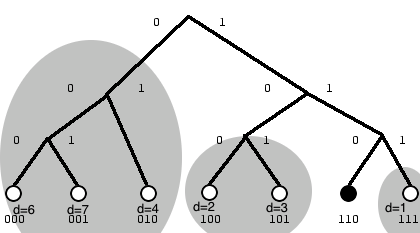
\includegraphics[width=0.5\textwidth]{images/tree}
  \caption{\label{tree}Nodes are leaves. $k$-buckets are increasingly large neighborhoods/subtrees.}
\end{figure}

These lists are known as $k$-buckets.
The peers inside each $k$-bucket are ordered by how recently they were seen, with the most recent encounters at the tail.
For small values of $i$, the $k$-buckets are probably going to be empty.
That is, the $0^{\mathrm{th}}$ $k$-bucket, which stores the peer that is one away, is almost certainly going to be empty; this is because the keyspace is so large that we will rarely see $k_1 \oplus k_2 = 1$.
In layman terms, nodes are going to be spread out, so the $k$-buckets that can store a wider range of nodes are more likely to be filled.

However, there is a limit to how large a $k$-bucket can get: that limit is determined by a system-wide parameter, $k$. Every time a node receives a request or reply, it updates its $k$-bucket for the sender. If the sender is already in the appropriate $k$-bucket, it moves to the tail of the list. If there are fewer than $k$ entries in the bucket, the sender moves to the tail as well. If the bucket is full, then the recipient node pings the least-recently seen node at the head of the list and waits for a response; if no response comes, the sender node is inserted at the list tail; but if the least-recently seen node responds, then it moves to the list tail and the sender node is discarded.

This least-recently seen eviction policy has two main advantages. First, it is a natural defense against flooding attacks, like DDoS, since the $k$-buckets are capped in size. Second, the preference for old contacts has been empirically shown to have availability benefits: the longer a node has been up, the more likely it is to stay up for another hour.

\subsubsection{Protocol}

\newcommand{\findNode}{}
\def\findNode/{{\sc find\_node}}
\newcommand{\findValue}{}
\def\findValue/{{\sc find\_value}}
\newcommand{\ping}{}
\def\ping/{{\sc ping}}
\newcommand{\store}{}
\def\store/{{\sc store}}

The Kademlia protocol is comprised of four main RPC calls: \ping/, \store/, \findNode/, and \findValue/.

The \ping/ RPC checks to see if a node is online and, as previously mentioned, is used when a $k$-bucket is full and a node wants the status of the least-recently seen peer in that bucket.

\store/ tells a node to store a \kv/ pair.

The \findNode/ RPC takes a 160-bit node ID as an argument and returns the $k$ nodes that are closest to the target ID. \findValue/ works much like \findNode/, except the recipient of a \findValue/ RPC will return a stored value if it has received a \store/ RPC for the key.

Underlying these RPCs is the most important and most complex operation in Kademlia: node lookup. This entails locating the $k$ nodes closest to a given node ID. The lookup initiator starts by picking $\alpha = 3$ nodes from its closest non-empty $k$-bucket (remember that the closest $k$-buckets will probably be empty) and then sends parallel, asynchronous \findNode/ RPCs to the $\alpha$ nodes. Following those \findNode/ RPCs, the initiator will become privy to new nodes and can query those. If a round of queries does not return a single node closer to the target node, then the initiator queries nodes that have not already been queried. The lookup ends when it can find nothing closer and when the $k$ closest nodes have all responded.

Node lookup is used in the \store/ RPC for replication. When a \kv/ pair is stored at a particular target node, it is also stored at the $k$ closest peers of that target node. Replica entries are kept fresh since nodes republish their \kv/ pairs on the hour, and since entries will expire after 24 hours to limit stale data. Finally, when node $a$ encounters another node $b$ that is closer to some of $a$'s \kv/ pairs, $a$ replicates them over to $b$.

\section{Entangled}
\newcommand{\delete}{}
\def\delete/{{\sc delete}}
We use Entangled, a Python implementation of the Kademlia DHT.
In addition, Entangled also features a \delete/ RPC for deleting \kv/ pairs from the DHT, a fully distributed peer-to-peer tuple space, and keyword-based operations, such as publish, search and remove.



\section{Design Challenges}
\subsection{Replication}
\subsection{Synchronization}



\section{Implementation}
Our implementation of this system began with reading through the source code and limited documentation of the various pieces of what was to be in our final system and understanding how each of the pieces worked and interacted. Running the actual server for the nodes is an implementation called tornado, that handles the creation of a webserver and the majority of the transport layer. The OpenBazaar p2p interactions run on a network library called zeromq that handles most of the peer-to-peer setup and network maintenance between the nodes in the system. The system is designed fairly sensibly, with the various cryptographic components separated out into seperate modules from the core market interactions. The website itself is accessed through a browser, typically at {{\sc localhost:8888}}, and is a fairly straightforward html and javascript site that allows for updates to your own market and provides a GUI for interaction with other sites in the network.

\subsection{Current Implementation}
The current implementation is evolving rapidly with contributions from the open-source community, but the basic structure of the codebase has remained relatively the same. The majority of the market interactions are implemented in the node folder. Files within here create the various networking compnents, including event handlers and protocol implementations, that allow the market to function on its lowest layer. 

\subsection{Additions}
% describe modifications to market, run, tornadoloop, etc

\subsection{Issues}
Once we had gotten over the hurdle of understanding how the various components of the existing codebase functioned, the codebase implementation of handling the API calls was fairly straightforward



\section{Evaluation}




\section{Conclusion}



\end{document}
